% Teto: 2.500 palavras no total (4.1: 650; 4.2: 400 e uma tabela; 4.3: 650 e uma tabela;
% 4.4: 600). Fonte: 4.1 e Limitações do .docx (PR 56), tarefas 93 e 95, resultados dos agentes.
\section{Resultados e discussão}

\subsection{Classificador}

\pendente{4.1 do .docx, com as Tabelas 1 e 2 e a figura do recall com o pcap fora do treino
(PR 57)}

\begin{figure}[htb]
	\centering
	\caption{\pendente{legenda da matriz de confusão}}
	\label{fig:matriz}
	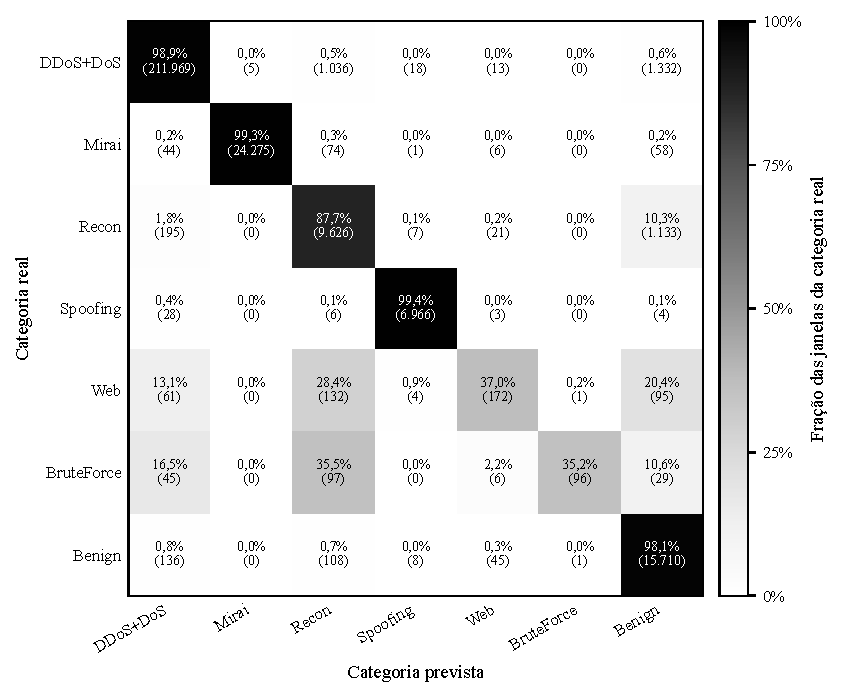
\includegraphics[width=0.8\textwidth]{matriz_confusao.pdf}
	\legend{Fonte: os autores.}
\end{figure}

\subsection{Tráfego fora do CICIoT2023}

\pendente{a casa, o IoT-23 e o CICIoMT2024 numa tabela só (tarefas 93 e 95)}

\subsection{Agentes}

\pendente{as três configurações (local, nuvem e híbrida): veredito, recomendação contra o
gabarito, custo e latência}

\subsection{Limitações}

\pendente{de 24 itens para 8 a 10}
